\documentclass[11pt]{article}
\usepackage[margin=1in]{geometry}
\usepackage{amsmath,amssymb,amsfonts}
\usepackage{booktabs}
\usepackage{graphicx}
\graphicspath{{../}}
\usepackage{hyperref}

\title{Basin Stability Protocol for Phase Diagram Measurement\\
       in Continuous Dense Associative Memory}
\author{}
\date{}

\begin{document}
\maketitle

\section{Overview}

We measure the retrieval phase boundaries of Dense Associative Memory (DAM) on the $N$-sphere $S^{N-1}(\sqrt{N})$ with exponential capacity $P = e^{\alpha N}$, for two energy kernels:
\begin{itemize}
    \item \textbf{LSE} (Gaussian / log-sum-exp):
    $H(\mathbf{x}) = -\beta_{\mathrm{net}}^{-1}\ln\sum_{\mu} e^{-\beta_{\mathrm{net}} N(1 - \phi^\mu)}$,
    \quad $\beta_{\mathrm{net}} = 1$,
    \item \textbf{LSR} (Epanechnikov / log-sum-ReLU):
    $H(\mathbf{x}) = -(N/b)\ln\sum_{\mu}[1 - b(1 - \phi^\mu)]_+$,
    \quad $b = 2 + \sqrt{2} \approx 3.414$,
\end{itemize}
where $\phi^\mu = \boldsymbol{\xi}^\mu \!\cdot\! \mathbf{x}/N$ is the alignment with pattern~$\mu$.

The theoretical phase boundaries are derived in the thermodynamic limit $N \to \infty$ at fixed load $\alpha$.
Monte Carlo validation at finite $N$ must maintain the exponential-capacity relationship $P = e^{\alpha N}$ at each grid point, which is achieved through an adaptive-$N$ scheme.

Instead of measuring the thermal equilibrium alignment, we adopt a \emph{basin stability} approach: \textit{Is the retrieval basin stable against finite perturbations?}
The system is initialized with controlled random alignment $\varphi_{\mathrm{init}} \in [0.75, 1.0]$ and relaxed via Metropolis dynamics.
The final alignment measures whether the energy landscape pulls the state back toward the target ($\varphi \to 1$, stable basin) or fails to do so ($\varphi$ drops, unstable basin).
This requires only enough dynamics to reveal the convergence direction---not full exploration of the Boltzmann distribution---making it robust at all temperatures.

\section{Adaptive-$N$ Design}

The theoretical predictions hold at fixed $\alpha = \ln P / N$.
For each $\alpha$, the network dimension is set by
\begin{equation}
    N(\alpha) = \left\lfloor \frac{\ln P(\alpha)}{\alpha} \right\rceil,
\end{equation}
ensuring $P \approx e^{\alpha N}$ exactly at every grid point.
The pattern count $P(\alpha)$ follows a power-law interpolation
\begin{equation}
    P(\alpha) = \bigl[\text{linspace}(P_{\min}^{1/\gamma},\; P_{\max}^{1/\gamma},\; n_\alpha)\bigr]^\gamma,
    \qquad \gamma = 10,
\end{equation}
with $P_{\min} = 20{,}000$ and $P_{\max} = 500{,}000$.
The large exponent $\gamma = 10$ concentrates the pattern distribution toward $P_{\max}$, providing large $N$ (good convergence to thermodynamic limit) at low $\alpha$ while keeping memory requirements manageable at high $\alpha$.

This adaptive scheme avoids the two failure modes of fixed-$N$ simulations:
(i)~\emph{pattern capping}, which collapses the effective load above a cutoff $\alpha$, and
(ii)~\emph{insufficient patterns} at low $\alpha$, where the noise floor never forms.

\section{Monte Carlo Protocol}

The protocol has two cleanly separated phases for each $(\alpha, T)$ point.

\subsection{Initialization}

For each trial $t$ and temperature slot $j$, a random initial alignment $\varphi_{\mathrm{init}} \sim \mathrm{Uniform}(0.75, 1.0)$ is drawn.
The initial state is constructed as
\begin{equation}
    \mathbf{x}_{\mathrm{init}} = \varphi_{\mathrm{init}}\, \boldsymbol{\xi}^1
    + \sqrt{1 - \varphi_{\mathrm{init}}^2}\;\sqrt{N}\; \hat{\mathbf{u}}_\perp,
\end{equation}
where $\hat{\mathbf{u}}_\perp$ is a random unit vector orthogonal to $\boldsymbol{\xi}^1$ (obtained via Gram--Schmidt).
This guarantees $\|\mathbf{x}_{\mathrm{init}}\| = \sqrt{N}$ and $\boldsymbol{\xi}^1 \!\cdot\! \mathbf{x}_{\mathrm{init}}/N = \varphi_{\mathrm{init}}$ exactly.
For LSR, $\varphi_{\mathrm{init}} \geq 0.75 > \varphi_c = (b-1)/b \approx 0.707$ ensures the initial state lies within the kernel support.

\subsection{Phase 1: Equilibration (unmeasured)}

$N_{\mathrm{eq}} = 2^{14} = 16{,}384$ Metropolis--Hastings steps are executed without recording any observables.
This phase discards the initial transient, allowing the system to settle into the basin's steady state (or leave the basin if it is unstable at the given $T$ and $\alpha$).

\subsection{Phase 2: Sampling (measured)}

$N_{\mathrm{samp}} = 2^{12} = 4{,}096$ additional steps are executed, and the alignment $\varphi_s = \boldsymbol{\xi}^1 \!\cdot\! \mathbf{x}_s / N$ is accumulated at every step.
The time-averaged alignment for trial $t$ is
\begin{equation}
    \bar{\varphi}_t = \frac{1}{N_{\mathrm{samp}}} \sum_{s=1}^{N_{\mathrm{samp}}} \varphi_t^{(s)}.
\end{equation}

By measuring $\varphi$ only during the sampling phase, the observable is not polluted by the initial transient from $\varphi_{\mathrm{init}}$.

\subsection{Disorder averaging}

The reported alignment at each grid point is the average over $n_{\mathrm{trials}}(\alpha)$ independent trials, each with a fresh random pattern set:
\begin{equation}
    \varphi(\alpha, T) = \frac{1}{n_{\mathrm{trials}}} \sum_{t=1}^{n_{\mathrm{trials}}} \bar{\varphi}_t.
\end{equation}
The trial count is adaptive: $n_{\mathrm{trials}} = 512$ at $\alpha_{\min} = 0.01$ (where patterns are cheap) and decreases linearly to $n_{\mathrm{trials}} = 64$ at $\alpha_{\max} = 0.55$ (where each trial involves $P \approx 500{,}000$ patterns).

\subsection{Metropolis--Hastings on the $N$-sphere}

Both LSE and LSR use the same update rule:
\begin{enumerate}
    \item Propose $\mathbf{x}' = \mathbf{x} + \sigma\,\boldsymbol{\eta}$, \quad $\boldsymbol{\eta} \sim \mathcal{N}(0, I_N)$, \quad $\sigma = \max(0.1,\; 2.4/\sqrt{N})$.
    \item Project: $\mathbf{x}' \leftarrow \sqrt{N}\,\mathbf{x}'/\|\mathbf{x}'\|$.
    \item Accept with probability $\min(1,\, e^{-\Delta H / T})$.
\end{enumerate}
For LSR, proposals that move outside all pattern supports ($H = +\infty$) are automatically rejected, enforcing the hard-wall constraint.

\section{GPU Implementation}

\subsection{Parallelization strategy}

The simulation processes $\alpha$ values sequentially (or in memory-limited chunks), while all $n_T$ temperatures and $n_{\mathrm{trials}}$ trials are batched on the GPU simultaneously.
For each $\alpha_i$, the state array has shape $[N_i \times n_T \times n_{\mathrm{trials}}]$, and the Metropolis step operates via batched CUBLAS \texttt{gemm\_strided\_batched} for the energy computation.

\subsection{Memory management}

The adaptive scheme produces $N$ ranging from $\sim\!24$ (at $\alpha = 0.55$) to $\sim\!990$ (at $\alpha = 0.01$), with correspondingly different memory footprints.
The code estimates memory per $\alpha$ and groups values into chunks fitting within the target GPU memory budget (${\sim}43$~GB on a 50~GB device), processing one chunk at a time with explicit GPU memory reclamation between chunks.

\subsection{Reproducibility}

Pattern generation uses a deterministic seed ($42 + i_\alpha$) per $\alpha$ index, ensuring full reproducibility across runs.
The same pattern set is shared across all temperatures for a given $\alpha$, isolating thermal effects from quenched-disorder fluctuations.

\section{Interpretation of Results}

The measured $\varphi(\alpha, T)$ has the following physical interpretation:
\begin{itemize}
    \item $\varphi \approx 1$: The retrieval basin is stable---perturbations of $\varphi_{\mathrm{init}} \in [0.75, 1.0]$ converge back to the target pattern.
    \item $\varphi \approx 0$: The retrieval basin is absent or unstable---the system escapes to a disordered state.
    \item Intermediate $\varphi$: A mixture of successful and failed retrievals across trials, indicating marginal basin stability.
\end{itemize}

The phase boundary $\alpha_c(T)$, where basin stability is lost, is compared against the theoretical predictions:
\begin{align}
    \text{LSE (Eq.\,35):} \quad \alpha_c^{\mathrm{LSE}}(T) &= \tfrac{1}{2}\bigl[1 - f_{\mathrm{ret}}^{\mathrm{LSE}}(T)\bigr]^2, \\
    \text{LSR (Eq.\,39):} \quad \alpha_c^{\mathrm{LSR}}(T) &= \tfrac{1}{2}\bigl[1 - f_{\mathrm{ret}}^{\mathrm{LSR}}(T)\bigr]^2,
\end{align}
where $f_{\mathrm{ret}}(T)$ is the retrieval free energy density obtained from the saddle-point equations (Eqs.\,33 and~36).

\section{Boltzmann Equilibrium Within the Retrieval Basin}

A measured alignment $\varphi \ll 1$ does \emph{not} necessarily indicate retrieval failure.
Even when the retrieval basin is the unique thermodynamic state (no spin-glass competition), the alignment at finite temperature is reduced by thermal fluctuations and takes the Boltzmann-averaged value $\varphi_{\mathrm{eq}}(T) < 1$.
This effect is purely statistical-mechanical: the density of states on $S^{N-1}(\sqrt{N})$ strongly favors lower alignments, and only the energy gradient near the target pattern counteracts this entropy.

\subsection{Single-basin Boltzmann average}

Consider a single stored pattern $\boldsymbol{\xi}^1$ (the dominant term in the retrieval basin).
For the LSR kernel, the internal energy density is (Eq.\,57)
\begin{equation}
    u(\varphi) = -b^{-1}\ln\bigl[1 - b(1-\varphi)\bigr], \qquad \varphi > \varphi_c = 1 - 1/b,
\end{equation}
with a hard wall at $\varphi_c = (b-1)/b \approx 0.707$.
The density of states on the $N$-sphere at alignment $\varphi$ is
\begin{equation}
    \rho(\varphi) \propto (1 - \varphi^2)^{(N-3)/2}.
\end{equation}
This function is sharply peaked near $\varphi = 0$ for large $N$: the vast majority of the sphere's surface area lies at low alignment.

The thermal average within the retrieval basin is
\begin{equation}\label{eq:boltzmann-avg}
    \langle\varphi\rangle_T
    = \frac{\displaystyle\int_{\varphi_c}^{1} \varphi\; \rho(\varphi)\; e^{-N\,u(\varphi)/T}\, \mathrm{d}\varphi}
           {\displaystyle\int_{\varphi_c}^{1} \rho(\varphi)\; e^{-N\,u(\varphi)/T}\, \mathrm{d}\varphi}.
\end{equation}
For LSE, the same integral applies with $u(\varphi) = 1 - \varphi$ (the Gaussian energy density) and the lower limit replaced by $-1$.

\subsection{Physical mechanism}

The integral~\eqref{eq:boltzmann-avg} is determined by the competition between two factors:
\begin{itemize}
    \item The \textbf{energy} $u(\varphi)$ favors $\varphi \to 1$ (the target pattern is the energy minimum).
    \item The \textbf{entropy} $\rho(\varphi)$ favors $\varphi \to 0$ (exponentially more states at lower alignment).
\end{itemize}
At $T = 0$, energy dominates and $\langle\varphi\rangle \to 1$.
As $T$ increases, entropy becomes more important and $\langle\varphi\rangle$ decreases monotonically.
For LSR with $b = 2 + \sqrt{2}$, the alignment drops from ${\approx}\,1$ at $T \to 0$ to ${\approx}\,0.78$ at $T = 2$---even though the retrieval basin remains the unique stable state at all temperatures (for $\alpha < \alpha_{\mathrm{th}}$).
For LSE, the Boltzmann average follows Eq.\,33: $\varphi_{\mathrm{LSE}}(T) = \tfrac{1}{2}[-T + \sqrt{T^2 + 4}]$, which drops more steeply (reaching ${\approx}\,0.65$ at $T = 2$).

In the thermodynamic limit ($N \to \infty$), the Boltzmann integral is dominated by its saddle point, recovering the equilibrium alignment from the mean-field equations (Eq.\,33 for LSE, Eq.\,36 for LSR).
At finite $N$, the integral~\eqref{eq:boltzmann-avg} is evaluated numerically using the log-sum-exp trick for stability, with a fine grid of $5{,}000$ points over $[\varphi_c, 1]$.

\subsection{Monte Carlo validation}

Figure~\ref{fig:boltzmann} compares the Boltzmann prediction~\eqref{eq:boltzmann-avg} with Monte Carlo data for the LSR kernel at $\alpha = 0.1$ (well inside the retrieval phase, below $\alpha_{\mathrm{th}} \approx 0.25$).
For $T \gtrsim 0.2$, the MC data agrees with the Boltzmann integral to within ${\sim}\,0.5\%$ (RMS), confirming that the simulation correctly samples the thermal equilibrium within the single retrieval basin.

This comparison has an important implication for interpreting the basin stability maps:
values of $\varphi \approx 0.8$ in the retrieval region do not indicate partial retrieval failure---they are the \emph{expected} thermal equilibrium values at the given temperature.
The physically meaningful observable is the \emph{deviation} $\varphi(\alpha, T) - \varphi_{\mathrm{eq}}(T)$, which isolates the effect of pattern interference from thermal broadening (see the difference maps).

\begin{figure}[h]
\centering
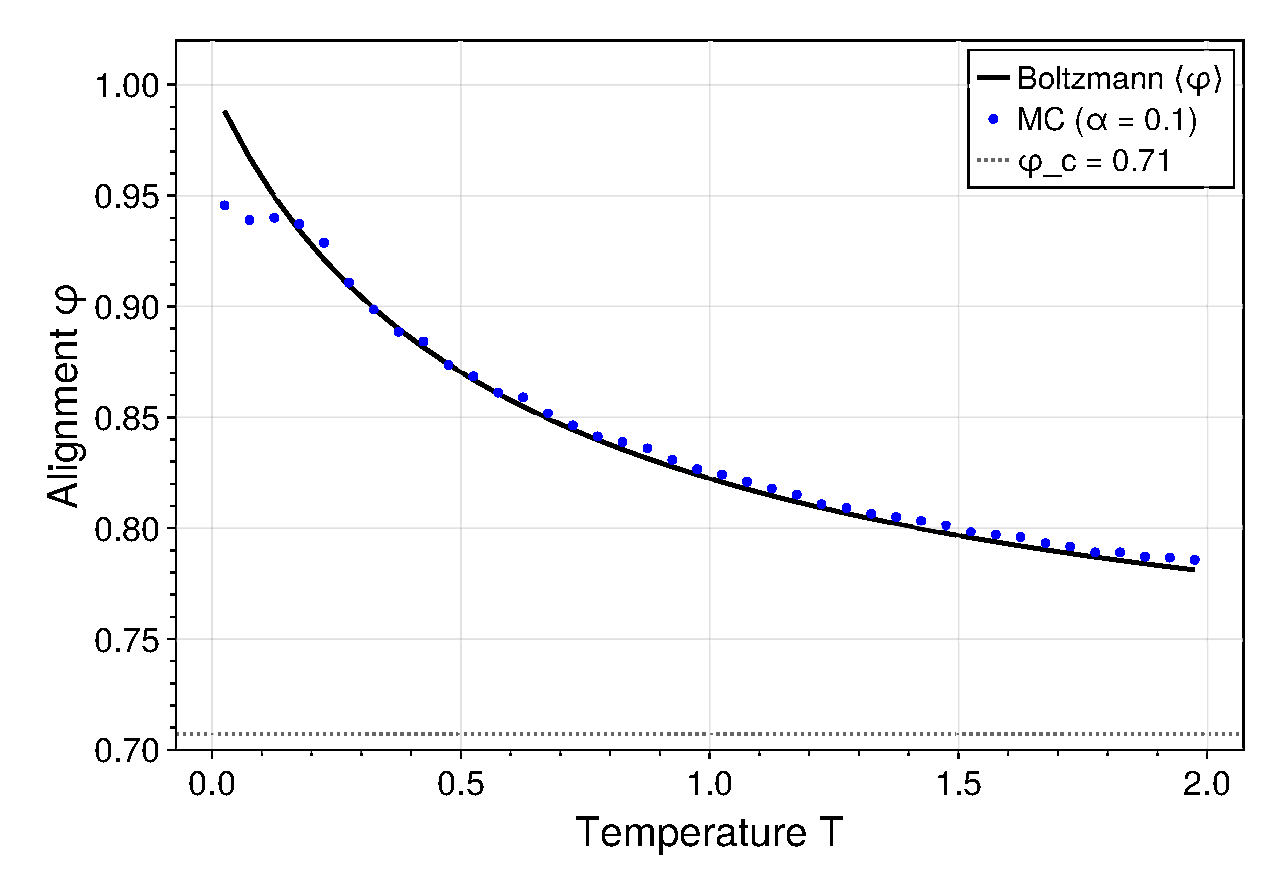
\includegraphics[width=0.45\columnwidth]{boltzmann_comparison_alpha01.eps} \hspace{5mm} 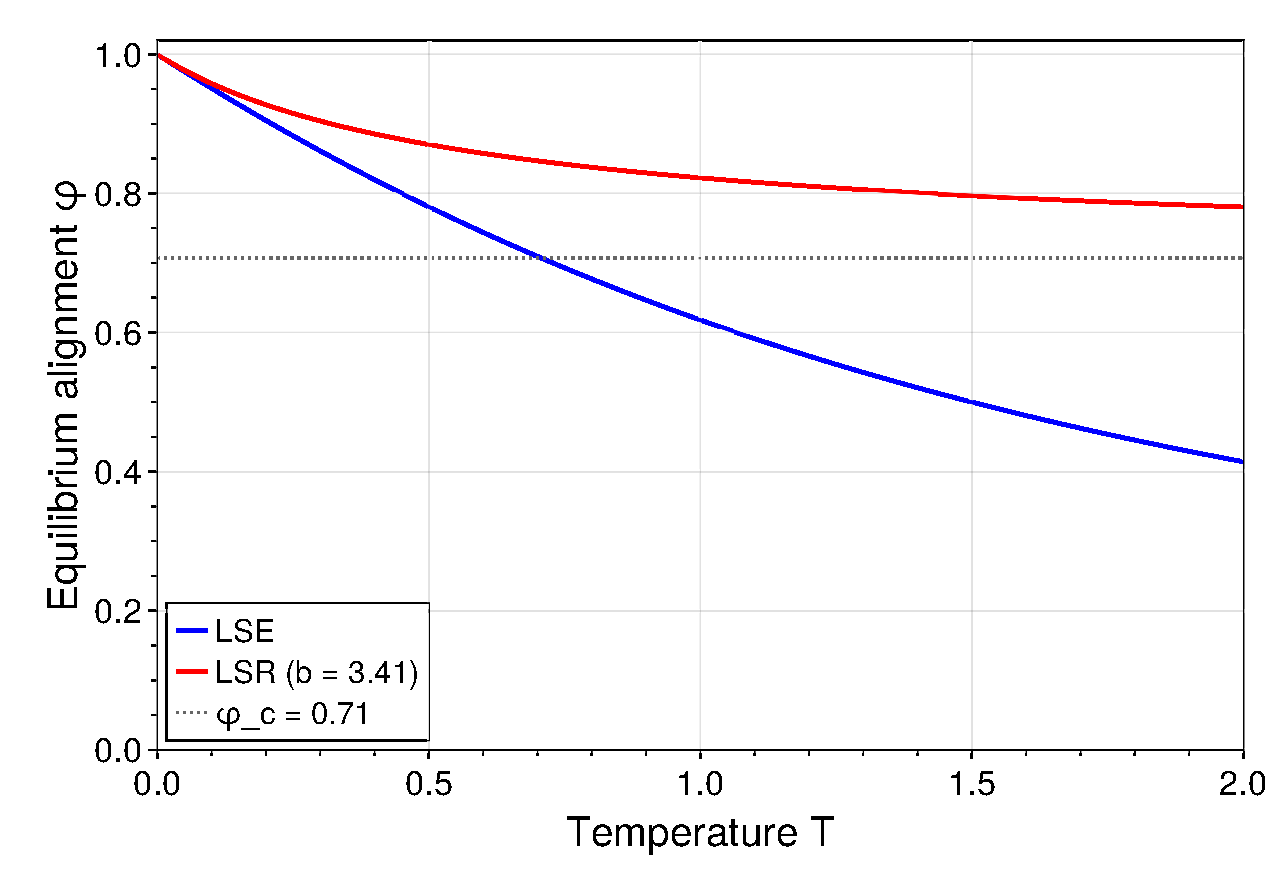
\includegraphics[width=0.45\columnwidth]{phi_eq_vs_T_prod.eps}
\caption{\textit{Left:} Boltzmann equilibrium within the LSR retrieval basin at $\alpha = 0.1$.
Solid curve: theoretical $\langle\varphi\rangle_T$ from Eq.\,\eqref{eq:boltzmann-avg}.
Blue circles: Monte Carlo data.
Dotted line: hard-wall threshold $\varphi_c \approx 0.71$.
The alignment decreases monotonically with $T$ due to the entropy--energy competition, even though the retrieval basin is perfectly stable at this load.
\textit{Right:} Equilibrium alignment $\varphi_{\mathrm{eq}}(T)$ for both kernels.
LSE (Eq.\,33, blue) drops more steeply than LSR (Eq.\,37, red), which is bounded below by the hard wall at $\varphi_c$.}
\label{fig:boltzmann}
\end{figure}

\section{Simulation Parameters}

\begin{table}[h]
\centering
\caption{Basin stability Monte Carlo parameters.
Both LSE and LSR use identical settings; only the energy function differs.}
\label{tab:mc-params}
\small
\begin{tabular}{ll}
\toprule
Parameter & Value \\
\midrule
\multicolumn{2}{l}{\textit{Energy models}} \\[2pt]
LSE parameter       & $\beta_{\mathrm{net}} = 1$ \\
LSR parameter       & $b = 2 + \sqrt{2} \approx 3.414$ \\[4pt]
\multicolumn{2}{l}{\textit{Phase-space grid}} \\[2pt]
$\alpha$ grid       & $0.01{:}0.01{:}0.55$ \;(55 values) \\
$T$ grid            & $0.025{:}0.05{:}2.0$, linear \;(40 values) \\
$P$ range           & $20{,}000$--$500{,}000$ \;(power-law, $\gamma = 10$) \\
$N$ range           & ${\sim}\,24$--$990$ \;(adaptive, $N = \ln P / \alpha$) \\[4pt]
\multicolumn{2}{l}{\textit{Monte Carlo protocol}} \\[2pt]
Initialization      & $\varphi_{\mathrm{init}} \!\sim\! \mathrm{U}(0.75,\, 1.0)$ \\
Equilibration       & $2^{14} = 16{,}384$ steps (unmeasured) \\
Sampling            & $2^{12} = 4{,}096$ steps ($\varphi$ measured) \\
Trials              & $512 \to 64$ (adaptive, more at low $\alpha$) \\
Step size           & $\sigma = \max(0.1,\; 2.4/\sqrt{N})$ \\
Update              & Metropolis on $S^{N-1}(\sqrt{N})$ \\[4pt]
\multicolumn{2}{l}{\textit{Implementation}} \\[2pt]
GPU parallelism     & All $T$ \& trials batched; sequential over $\alpha$ \\
Precision           & Float32 \\
Quenched disorder   & One fresh pattern set per trial \\
Observable          & $\varphi = \langle \boldsymbol{\xi}^1 \!\cdot\! \mathbf{x}\rangle / N$ \\
\bottomrule
\end{tabular}
\end{table}

\end{document}
